\documentclass[11pt,a4paper]{article}
\usepackage[T1]{fontenc}
\usepackage[utf8]{inputenc}
\usepackage{lmodern}
\usepackage[margin=25mm,headheight=14pt]{geometry}
\usepackage{amsmath,amssymb,amsthm,mathtools}
\usepackage{microtype}
\usepackage{graphicx,xcolor,booktabs,tabularx,array}
\usepackage{placeins}
\usepackage{enumitem}
\usepackage{fancyhdr}
\usepackage[numbers,sort&compress]{natbib}
\usepackage[colorlinks=true,linkcolor=blue!45!black,citecolor=blue!45!black,urlcolor=blue!45!black]{hyperref}
\usepackage{bookmark}
\definecolor{ink}{HTML}{18374D}
\definecolor{teal}{HTML}{207D87}
\definecolor{pale}{HTML}{EDF5F6}
\usepackage{titlesec}
\titleformat{\section}{\large\bfseries\color{ink}}{\thesection}{.7em}{}
\titleformat{\subsection}{\normalsize\bfseries\color{ink}}{\thesubsection}{.7em}{}
\setlength{\parskip}{5pt}
\setlength{\parindent}{0pt}
\setlength{\emergencystretch}{2em}
\setlist{nosep,leftmargin=1.5em}
\newtheorem{theorem}{Theorem}[section]
\newtheorem{lemma}[theorem]{Lemma}
\newtheorem{proposition}[theorem]{Proposition}
\theoremstyle{definition}
\newtheorem{definition}[theorem]{Definition}
\newcommand{\R}{\mathbb R}
\newcommand{\Vol}{\operatorname{Vol}}
\newcommand{\Area}{\operatorname{Area}}
\newcommand{\conv}{\operatorname{conv}}
\graphicspath{{figures/}}
\pagestyle{fancy}
\fancyhf{}
\fancyhead[L]{\small\color{ink}Convex covers of unit space curves}
\fancyhead[R]{\small 19 November 2026}
\fancyfoot[C]{\small\thepage}
\hypersetup{pdftitle={Convex containers for every unit-length space curve},pdfauthor={Research report prepared for Vladimir Reshetnikov},pdfsubject={Three-dimensional Moser worm problem; rigorous upper and lower bounds}}

\begin{document}
\hypersetup{pageanchor=false}
\begin{titlepage}
\vspace*{7mm}
{\small\sffamily\color{teal}GEOMETRIC RESEARCH REPORT\par}
\vspace{5mm}
{\huge\bfseries\color{ink}Convex containers for every\\[2mm]unit-length space curve\par}
\vspace{5mm}
{\large The three-dimensional sleeping-bag problem\par}
\vspace{7mm}
Prepared for Vladimir Reshetnikov\hfill 19 November 2026
\vspace{9mm}

\colorbox{pale}{\parbox{\dimexpr\textwidth-2\fboxsep\relax}{%
\vspace{2mm}
\textbf{Answer.} The exact optimum is not known. For the minimum volume
$V_3$ of a compact convex body containing a translated and properly rotated
copy of every rectifiable curve of length one, this report establishes
\[
\boxed{\frac{3}{220}\le V_3\le\frac{\pi}{54}}
\qquad
\boxed{0.0136363636\ldots\le V_3\le0.0581776417\ldots.}
\]
The lower bound has an elementary proof and an exact finite certificate.
The upper bound is an explicit ellipsoidal sector, deduced from two
published geometric theorems. The minimum is attained, although its value
and an optimal body remain unidentified.
\vspace{2mm}
}}

\vspace{6mm}
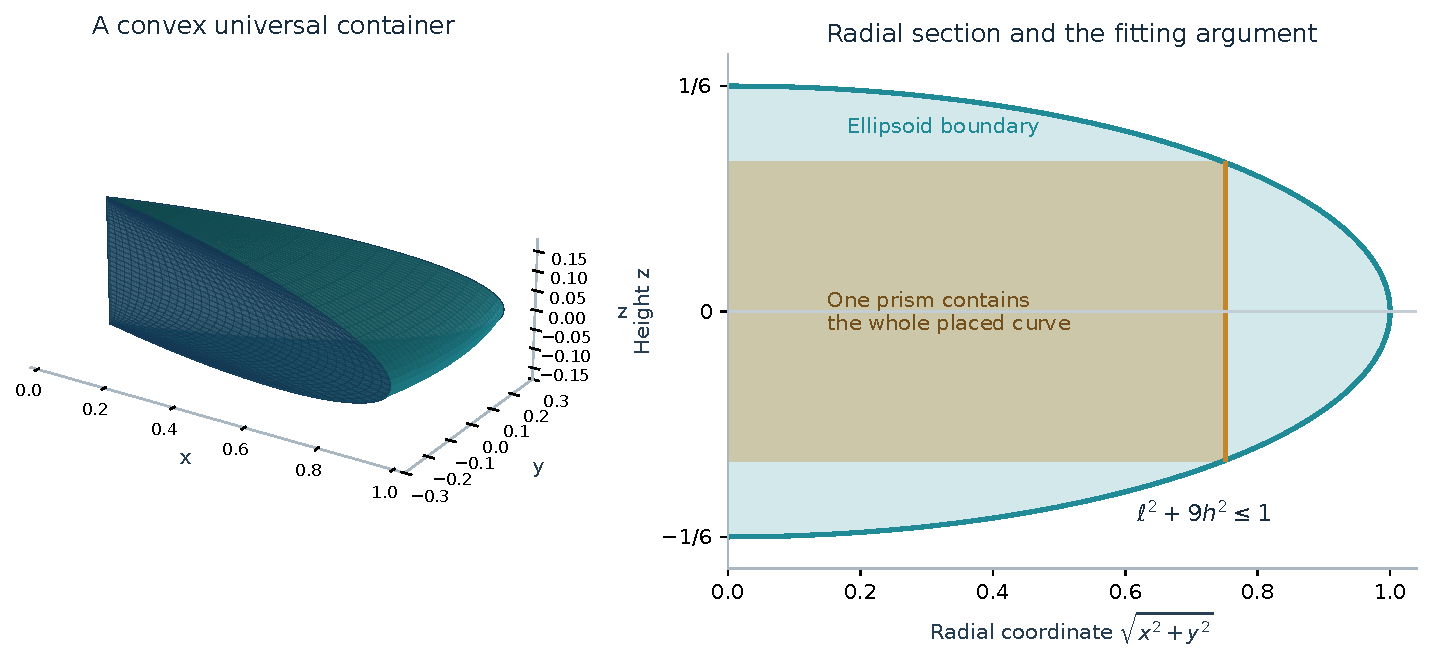
\includegraphics[width=\textwidth]{cover.pdf}

\vspace{3mm}
\textbf{Recent preprint.} A September 2026 planar-cover theorem would,
through the same lifting argument, improve the upper bound to
$0.0547404971558\ldots$. Its dependency and verification status are
stated separately in Section~\ref{sec:literature}.

\end{titlepage}

\pagenumbering{roman}
\hypersetup{pageanchor=true}
\tableofcontents
\clearpage
\pagenumbering{arabic}
\section{The precise optimization problem}\label{sec:problem}

A curve is a continuous rectifiable map $\gamma:[0,1]\to\R^3$.
Its length is
\[
 L(\gamma)=\sup_{0=t_0<\cdots<t_m=1}
 \sum_{i=1}^m\|\gamma(t_i)-\gamma(t_{i-1})\|.
\]
Corners, self-intersections, and retracing are allowed; retraced travel
contributes to the length. The trace is $\Gamma=\gamma([0,1])$.
All test curves used for the lower bounds are simple polygonal arcs or a
smooth simple helix, so those lower bounds also apply if one restricts
the question to simple curves.

Here a \emph{convex body} is a compact convex subset of $\R^3$ with nonempty
interior. A body $K$ is a universal cover for unit space curves if
\[
 \text{for every $\gamma$ with $L(\gamma)=1$, there exist}
 \quad Q\in SO(3),\ b\in\R^3
 \quad\text{such that}\quad Q\Gamma+b\subseteq K.
\]
The rotation and translation may depend on the curve. The curve is rigid:
its shape is unchanged by its placement. We seek
\[
 V_3=\inf\{\Vol(K):K\text{ is such a convex universal cover}\}.
\]
Section~\ref{sec:existence} proves that this infimum is a minimum.
This is the spatial counterpart of Moser's worm problem, studied under
the name ``sleeping bag for a baby snake'' in~\cite{HLW2001}.

\paragraph{Exactly one and at most one.}
The same bodies cover every curve of length at most one. Indeed, append
a straight segment of the missing length to an endpoint of a shorter
path. A placement of this extended unit path also places its original
subpath. This argument is about paths and does not require the extension
to be injective. The reverse implication is immediate.

\paragraph{Boundary and scale conventions.}
Containment includes the boundary of $K$, as is customary. If containment
strictly inside the body is demanded, arbitrarily small dilations about
an interior point preserve universality and make every contained trace
interior. Thus the infimum is unchanged, although attainment under that
stronger convention need not follow. For a different length $L>0$,
dilation gives
\[
 V_3(L)=L^3 V_3(1).
\]

\paragraph{Related questions that have different answers.}
The curve is not required to be closed. Closed unit loops have diameter at
most $1/2$, whereas this problem includes a straight unit segment.
Nor is this the problem of containing every set of diameter one:
the restriction to a trace of total length one is substantial.
Finally, maximizing $\Vol(\conv\Gamma)$ over individual curves gives a
lower bound for $V_3$, but does not produce a common container. A universal
body must fit many geometrically incompatible shapes.

\paragraph{How the report answers the question.}
The main result is a rigorous interval and a concrete feasible body,
not an asserted optimum. The upper bound combines published results;
the lower bound and its finite certificate are proved in full below.
The final literature section distinguishes a historical spatial bound,
our deductions from published theorems, and a newer preprint-dependent
improvement. The literature check was made on 19 November 2026.

% General lifting theorem; external inputs are stated, not reproved.
\section{Lifting a planar cover into three dimensions}\label{sec:lift}
The key construction applies to every convex planar universal cover, and
separates the geometric argument from the choice of a particular planar
cover. Planar congruences in the hypothesis may include reflections; the
resulting three-dimensional cover works using proper rotations alone.

\paragraph{External support-plane theorem.}
We use Wienholtz's alternating-support result in the form proved by
Ghomi~\cite[Corollary~3.2]{Ghomi2018}.
For a continuous space curve whose affine span is three-dimensional, there
are two parallel supporting planes and four parameter values
$t_0<t_1<t_2<t_3$ at which the curve meets the two planes alternately.
The curve lies in the slab between those planes. For a curve contained in a
plane, we will instead use that containing plane as a slab of width zero.
This is a nontrivial external theorem; the argument below is a deduction
from it. The planes need not realize the curve's minimum width.

\begin{theorem}[A planar cover produces a spatial cover]\label{thm:lift}
Let $C\subset\mathbb R^2$ be a compact convex set with nonempty interior,
containing the origin, which contains a congruent copy of every planar
rectifiable curve of length at most one. Set
\[
 f(z)=\sqrt{1-36z^2},\qquad -\frac16\le z\le\frac16,
\]
and define
\[
 K_C=\left\{(p,z)\in\mathbb R^2\times\mathbb R:
 |z|\le\frac16,\quad p\in f(z)C\right\}.
\]
Then $K_C$ is a convex body which contains a translated and properly rotated
copy of every rectifiable space curve of length at most one. Moreover,
\[
 \boxed{|K_C|=\frac29\operatorname{area}(C).}
\]
\end{theorem}
The assumption $0\in C$ entails no restriction on the area of a planar
cover: any chosen point of the cover may be translated to the origin.

\paragraph{Convexity and compactness.}
The function $f$ is continuous and concave on $[-1/6,1/6]$. Compactness of
$K_C$ follows from its representation as the continuous image of
$C\times[-1/6,1/6]$ under $(c,z)\mapsto(f(z)c,z)$. To check convexity,
take $(p_i,z_i)\in K_C$, write $p_i=f(z_i)c_i$ with $c_i\in C$, and let
$0\le\lambda\le1$. Put
\[
 z=(1-\lambda)z_1+\lambda z_2,\qquad
 a=(1-\lambda)f(z_1)+\lambda f(z_2).
\]
Convexity of $C$ gives
$(1-\lambda)p_1+\lambda p_2\in aC$; when $a=0$ this simply says that the
point is zero. Concavity gives $a\le f(z)$, and $0\in C$ implies
$aC\subseteq f(z)C$. Thus the convex combination belongs to $K_C$.
The product $(C/2)\times[-\sqrt3/12,\sqrt3/12]$ is contained in $K_C$,
so $K_C$ has nonempty interior even when the origin is a boundary point
of $C$.

\paragraph{Length of the two projections.}
Fix a curve $\gamma$ of length $L\le1$. A constant curve is immediate, so
assume $L>0$. Apply the support-plane theorem if the curve is nonplanar;
otherwise take a plane containing the curve. By a proper rigid motion,
put the resulting supporting planes at $z=-h/2$ and $z=h/2$, where $h\ge0$.
Write the transformed curve as $\gamma(s)=(p(s),z(s))$ and parametrize it
by arclength. Let $\ell$ be the length of the planar projection $p$, and
let $v$ be the total variation of $z$. The three alternating traversals
between the supporting planes give
\[
 v\ge3h.
\]
This inequality also holds in the planar case $h=0$.
Because an arclength parametrization is Lipschitz, its derivative exists
almost everywhere and the projection lengths satisfy
\[
 \ell=\int_0^L |p'(s)|\,ds,\qquad
 v=\int_0^L |z'(s)|\,ds.
\]
The triangle inequality for the integral of the two-dimensional vector
$(|p'(s)|,|z'(s)|)$ yields
\[
 \sqrt{\ell^2+v^2}
 \le \int_0^L\sqrt{|p'(s)|^2+|z'(s)|^2}\,ds=L\le1.
\]
Consequently
\[
 0\le h\le\frac13,
 \qquad \ell\le\sqrt{1-9h^2}.
\]
This is the essential link between the thickness of the chosen slab and
the amount of length left in its orthogonal projection. The quantity $h$
is the width of this chosen slab, not necessarily the minimum width over
all directions.

\paragraph{One rigid placement fits every height.}
If $\ell>0$, the planar universality of $C$, applied after scaling the
projection by $1/\ell$, supplies $A\in O(2)$ and $b\in\mathbb R^2$ such that
\[
 A p(s)+b\in\ell C\quad\hbox{for every }s.
\]
If $\ell=0$, the projection is a point; a translation sends it to the
origin, giving the same conclusion with $\ell C=\{0\}$.
For all points of the curve,
\[
 |z(s)|\le h/2\le1/6,
 \qquad
 f(z(s))\ge\sqrt{1-9h^2}\ge\ell.
\]
Since $0\in C$, we have $\ell C\subseteq f(z(s))C$. Hence this single
planar placement fits the entire three-dimensional curve into $K_C$ at
all heights simultaneously.

For completeness, even if the planar placement uses a reflection, the
three-dimensional placement can be chosen proper: put
$\varepsilon=\det A\in\{-1,1\}$ and use
\[
 (p,z)\longmapsto(Ap+b,\varepsilon z).
\]
Its linear part has determinant $(\det A)\varepsilon=1$, while replacing
$z$ by $-z$ preserves every slice of $K_C$. Composing with the initial
proper rigid motion proves the assertion without permitting reflections
of the physical space curve.

\paragraph{Volume.}
The section at height $z$ has area $f(z)^2\operatorname{area}(C)$. Thus
Cavalieri's principle gives
\[
 |K_C|=\operatorname{area}(C)
 \int_{-1/6}^{1/6}(1-36z^2)\,dz
 =\frac29\operatorname{area}(C).
\]

\subsection{An explicit ellipsoidal sector of volume \texorpdfstring{$\pi/54$}{pi/54}}
The planar theorem of Panraksa and Wichiramala~\cite{PW2021}
states that a circular sector of unit radius
and angle $\pi/6$ contains a congruent copy of every unit-length planar arc.
The statement for shorter arcs follows by extending the path to unit
length. Apply the lifting theorem to the sector
\[
 S=\{(\rho\cos\theta,\rho\sin\theta):
 0\le\rho\le1,\ |\theta|\le\pi/12\},
 \qquad \operatorname{area}(S)=\frac{\pi}{12}.
\]
Since $\tan(\pi/12)=2-\sqrt3$, its lift is the explicit convex body
\[
 \boxed{K_S=\left\{(x,y,z):
 x^2+y^2+36z^2\le1,\quad
 x\ge0,\quad |y|\le(2-\sqrt3)x\right\}.}
\]
It is the intersection of an ellipsoid with a $30$-degree dihedral wedge,
and
\[
 \boxed{|K_S|=\frac29\frac{\pi}{12}
 =\frac{\pi}{54}=0.05817764173314\ldots.}
\]
This is a rigorously justified feasible volume; the lifting argument does
not establish that it is the minimum. The more general theorem also shows
how any improved convex planar cover immediately gives a corresponding
three-dimensional upper bound.

\begin{figure}[htbp]
\centering
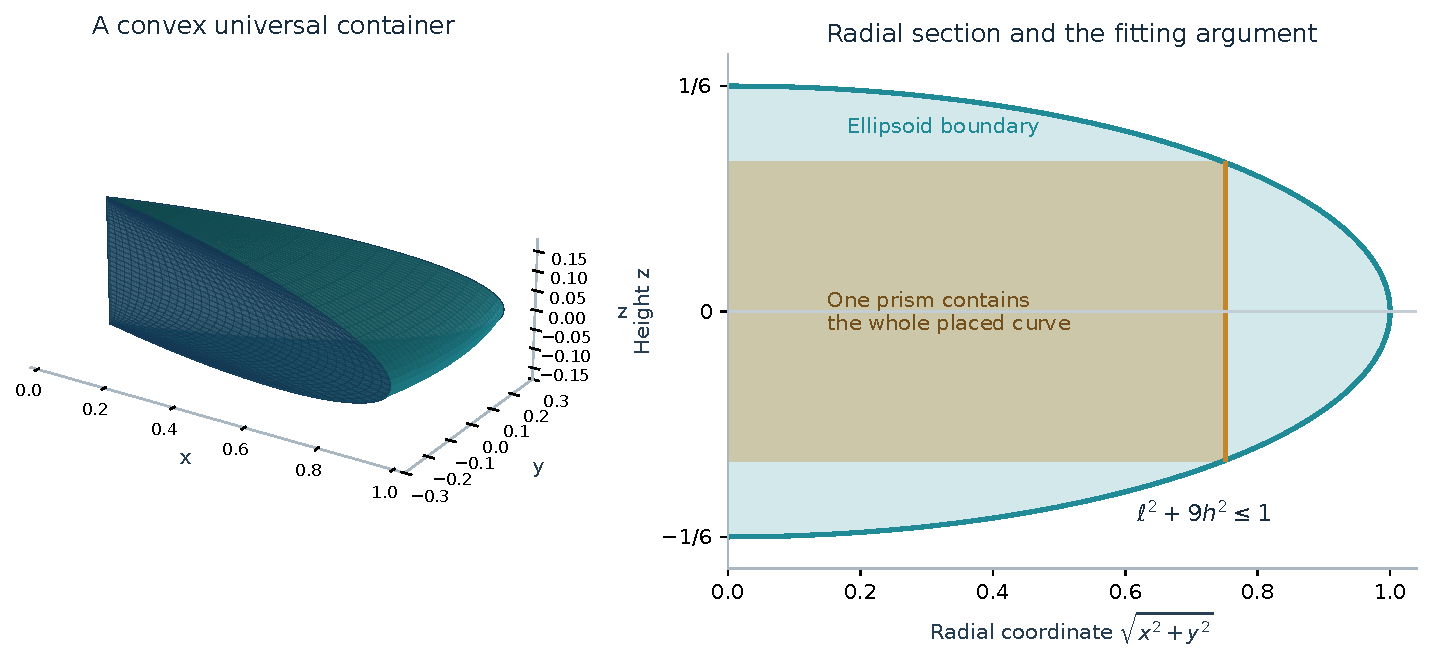
\includegraphics[width=\textwidth]{cover.pdf}
\caption{Left: the explicit universal convex body, an ellipsoid intersected with a $30^\circ$ dihedral wedge. Right: for any chosen alternating-support slab, one prism of height $h$ and planar scale $\ell$ fits inside the body. The figure illustrates the proof; containment is proved by the exact inequality $\ell^2+9h^2\le1$.}
\end{figure}

% A self-contained contribution to the main report.
\section{A lower bound from a regular tetrahedron and a unit segment}\label{sec:tetra}

Every convex universal cover must contain a congruent regular tetrahedron
of side length $1/3$: take a polygonal curve that visits all four vertices
along three consecutive edges.  It must also contain a unit line segment.
These two requirements combine to give a stronger bound than the volume
of either test curve's convex hull alone.

\begin{lemma}[A segment and a projection]\label{lem:fiber}
Let $K\subset\mathbb R^3$ be a convex body, let $u$ be a unit vector,
and suppose that $K$ contains a line segment of length $D$ parallel to $u$.
Writing $P_u$ for orthogonal projection onto $u^\perp$, we have
\[
 \operatorname{vol}_3(K)\geq
 \frac{D}{3}\operatorname{area}(P_uK).
\]
\end{lemma}
\begin{proof}
Set $B=P_uK$.  For $x\in B$, let $f(x)$ be the length of the fiber
$K\cap(x+\mathbb Ru)$.  Convexity shows that $f$ is nonnegative and
concave: convex combinations of two fiber intervals are contained in the
corresponding intermediate fiber.  At the projection $x_0$ of the given
segment, $f(x_0)\ge D$.  For $0\leq t\leq1$, concavity gives
\[
 f\bigl(t x_0+(1-t)x\bigr)\geq tD\qquad(x\in B).
\]
Consequently $\{f\geq tD\}$ contains $t x_0+(1-t)B$ and has area
at least $(1-t)^2\operatorname{area}(B)$.  Cavalieri's principle and
integration of the superlevel sets yield
\[
 \operatorname{vol}_3(K)=\int_B f(x)\,dx
 \geq D\operatorname{area}(B)\int_0^1(1-t)^2\,dt
 =\frac D3\operatorname{area}(B).
\]
The argument permits $x_0\in\partial B$ and fibers of zero length elsewhere.
\end{proof}

\begin{lemma}[Smallest shadow of a regular tetrahedron]
For a regular tetrahedron $T$ of side length $a$, every orthogonal planar
projection has area at least $a^2/(2\sqrt2)$.  Equality is attained when
the projection direction is parallel to an edge.
\end{lemma}
\begin{proof}
Put $b=a/(2\sqrt2)$ and choose vertices
\[
 b(1,1,1),\quad b(1,-1,-1),\quad
 b(-1,1,-1),\quad b(-1,-1,1).
\]
For a convex polytope, its projected area is half the sum of the projected
areas of its facets.  Indeed, except on sets of planar area zero, each
line through a point of the projection meets precisely one front facet
and one back facet.  For $u=(x,y,z)$ with $x^2+y^2+z^2=1$, the four
equal facet areas and their unit normals therefore give
\[
 \operatorname{area}(P_uT)=\frac{a^2}{8}\bigl(
 |x+y+z|+|x-y-z|+|-x+y-z|+|-x-y+z|\bigr).
\]
The expression in parentheses is invariant under permutations and sign
changes of the coordinates.  Thus assume $x\geq y\geq z\geq0$ and write
$s=x+y+z$.  The expression equals $4x$ if $x\geq y+z$, and $2s$
if $x\leq y+z$.

In the first case,
$1=x^2+y^2+z^2\leq x^2+(y+z)^2\leq2x^2$, so $4x\geq2\sqrt2$.
In the second, each coordinate is at most $s/2$, whence
$1=x^2+y^2+z^2\leq(s/2)(x+y+z)=s^2/2$, and again
$2s\geq2\sqrt2$.  This proves the claimed bound.  The direction
$u=(1,1,0)/\sqrt2$, parallel to one of the tetrahedron's edges,
attains equality.
\end{proof}

\begin{theorem}[An explicit universal-cover lower bound]
If a convex body $K\subset\mathbb R^3$ contains a translated and rotated
copy of every rectifiable curve of length $1$, then
\[
 \operatorname{vol}_3(K)\geq\frac{1}{54\sqrt2}
 =0.0130945700219731\ldots.
\]
\end{theorem}
\begin{proof}
Choose the direction $u$ of a unit segment in $K$.  Let $T\subset K$
be a regular tetrahedron of side $a=1/3$ obtained from the three-edge
test curve.  The two preceding lemmas imply
\[
 \operatorname{vol}_3(K)\geq\frac13\operatorname{area}(P_uK)
 \geq\frac13\operatorname{area}(P_uT)
 \geq\frac{a^2}{6\sqrt2}=\frac{1}{54\sqrt2}.
\]
The segment and tetrahedron may have arbitrary relative positions and
orientations.  The inequality uses no assumption about their placement.
\end{proof}

\paragraph{Status of this bound.}
The argument above is supplied as an independently verified elementary
bound, without a claim of historical priority or of being the best known
lower bound.  In particular, it is a lower bound for a common container,
not an identification of an optimal container.

% Self-contained strengthened lower-bound fragment.  Requires the segment/
% projection lemma in lower_bound.tex, or its equivalent in the main report.
\section{A stronger rational lower bound: 3/220}\label{sec:rational}

The same segment-and-projection argument can be strengthened using a
four-segment curve with a particularly convenient exact certificate.
No numerical optimization is needed in the proof.

\begin{lemma}[Finitely many directions suffice for a polytope's smallest shadow]
Let $P$ be a full-dimensional convex polytope with triangular facets.
For each facet, let $n_i$ be the cross product of two of its edge vectors,
in either orientation.  Then
\[
 A(u):=\operatorname{area}(P_uP)
 =\frac14\sum_i|n_i\cdot u|\qquad(\|u\|=1).
\]
The minimum of $A$ is attained at a direction parallel to $n_i\times n_j$
for some pair of linearly independent facet vectors.
\end{lemma}
\begin{proof}
The area formula follows by summing projected facet areas: a facet's area
is $\|n_i\|/2$, and the front and back facets each cover the projection
once almost everywhere.  Also $A(u)>0$ for every nonzero $u$, since
$P$ has interior.

Let $u$ minimize $A$. Suppose the facet vectors satisfying $n_i\cdot u=0$
span a space of dimension at most one. Choose a unit vector $v\perp u$
perpendicular to all these vanishing vectors, and set
\[
 u_\pm=\cos\varepsilon\,u\pm\sin\varepsilon\,v.
\]
For sufficiently small $\varepsilon>0$, every nonzero scalar product
retains its sign, and all zero scalar products stay zero. Therefore
\[
 A(u_+)+A(u_-)=2\cos\varepsilon\,A(u)<2A(u).
\]
One nearby direction would have smaller area, a contradiction. Thus
at a minimum two independent facet vectors vanish, so $u$ is parallel
to their cross product.
\end{proof}

Consider the five points
\[
\begin{array}{c|rrr}
i& p_{i,x}&p_{i,y}&p_{i,z}\\\hline
0& 3&0&0\\
1& 0&3&2\\
2&-3&0&4\\
3&0&-3&6\\
4&3&0&8
\end{array}
\]
and let $P=\operatorname{conv}\{p_0,\ldots,p_4\}$.
Every successive edge $p_ip_{i+1}$ has length $\sqrt{22}$.
Thus the polygonal curve through the scaled points
$p_i/(4\sqrt{22})$ has length exactly one.  Any convex universal
cover must contain a congruent copy of $P/(4\sqrt{22})$.

The facets and their cross-product vectors are as follows; the orientation
of a vector does not affect the projection formula.
\[
\begin{array}{c|c|rrr}
i&\text{facet}&n_{i,x}&n_{i,y}&n_{i,z}\\\hline
0&012&12&0&18\\
1&014&24&24&0\\
2&023&12&24&18\\
3&034&-24&24&0\\
4&124&-12&24&18\\
5&234&-12&0&18
\end{array}
\]
For completeness, these facets can be checked solely with integer
arithmetic: for every listed triple, the other two vertices lie strictly
on the same side of its plane; every unlisted nondegenerate triple has
vertices on both sides.  The accompanying program enumerates all ten
triples and performs exactly these checks.

For $v=n_i\times n_j\ne0$, the square of the projection area in direction
$u=v/\|v\|$ is the rational number
\[
 A(u)^2=
 \frac{\left(\sum_{k=0}^{5}|n_k\cdot v|\right)^2}{16\,v\cdot v}.
\]
All fifteen pairs are independent.  The complete list of distinct
values is short:
\[
\begin{array}{c|c|l}
A(u)^2&\text{multiplicity}&\text{pairs }(i,j)\\\hline
5184/25&1&(2,4)\\
216&2&(1,4),(2,3)\\
2592/11&6&(0,3),(0,4),(1,2),(1,5),(2,5),(3,4)\\
324&1&(1,3)\\
5184/13&2&(0,2),(4,5)\\
5832/11&2&(0,1),(3,5)\\
576&1&(0,5)
\end{array}
\]
These are exact rational calculations.  The minimum is $5184/25$,
so the smallest shadow of $P$ has area $72/5$.  It occurs in direction
$(0,-3,4)/5$, proportional to $n_2\times n_4$.
Scaling areas by $(4\sqrt{22})^{-2}=1/352$ gives
\[
 \min_{\|u\|=1}\operatorname{area}
 \left(P_u\left(\frac{P}{4\sqrt{22}}\right)\right)
 =\frac{72}{5\cdot352}=\frac9{220}.
\]

\begin{theorem}[Rational lower bound]
Every convex body that contains a translated and rotated copy of every
rectifiable space curve of length one has volume at least
\[
 \boxed{\frac3{220}=0.013636363636\ldots.}
\]
\end{theorem}
\begin{proof}
The body contains both a unit segment, in some direction $u$, and a
congruent copy of $P/(4\sqrt{22})$.  Its projection onto $u^\perp$
therefore has area at least $9/220$, irrespective of the relative
orientation of the two test curves.  The segment-and-projection lemma
gives volume at least $(1/3)(9/220)=3/220$.
\end{proof}

\paragraph{Reproducibility and scope.}
The file \texttt{code/verify\_lower\_bound.py} checks the edge lengths,
all supporting facets, the complete list of projection directions,
and the final bound using only integers and exact rational arithmetic
from the Python standard library.  The finite-direction lemma above
supplies the global mathematical justification; the certificate is
not a sampling experiment.  No claim of historical priority or
best-known status is made for this lower bound.

\begin{figure}[htbp]
\centering
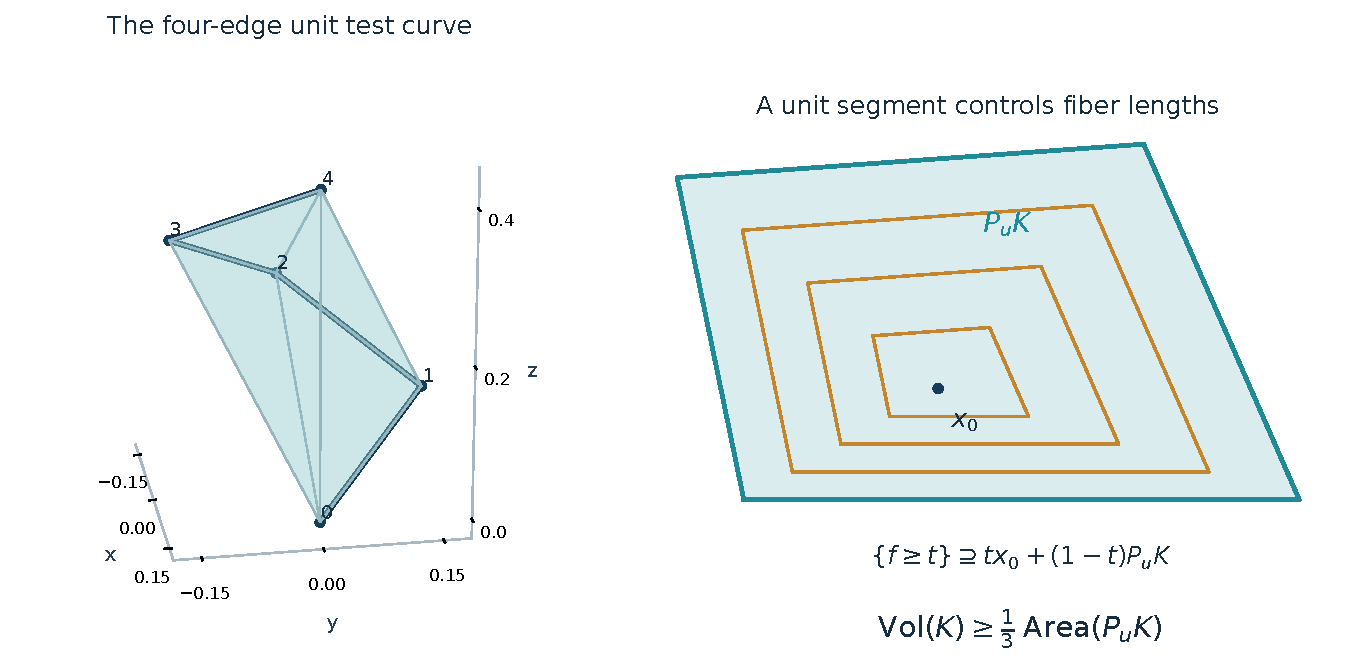
\includegraphics[width=\textwidth]{lower_bound.pdf}
\caption{Left: the four-edge test curve and its convex hull after normalization to length one. Right: a schematic illustration of the concave-fiber argument in Lemma~\ref{lem:fiber}. The nested copies of the shadow give a lower bound for every height superlevel set.}
\end{figure}

\FloatBarrier
\section{A minimum exists}\label{sec:existence}
We take a convex body to mean a compact convex subset of $\mathbb R^3$
with nonempty interior. Let $\mathcal U$ be the class of bodies containing,
for each rectifiable curve of length at most one, a copy obtained by a
translation and a proper rotation. The infimum
\[
 V_3 = \inf_{K\in\mathcal U}|K|
\]
is a minimum.

First, $\mathcal U$ is nonempty: every unit-speed curve on $[0,1]$ is
within distance $1/2$ of its point at parameter $1/2$, so the ball of radius
$1/2$ is universal. Shorter curves can be extended to length one.
Next consider the polygonal curve that traverses three successive edges
of a regular tetrahedron $T$ of edge length $a=1/3$. It has length one
and visits all four vertices, so its convex hull is $T$. This tetrahedron
has volume $a^3/(6\sqrt2)$ and surface area $\sqrt3a^2$; consequently
its insphere has radius
\[
 r_0=\frac{3|T|}{\operatorname{area}(\partial T)}
 =\frac{a\sqrt6}{12}=\frac{\sqrt6}{36}>0.
\]
Every universal body contains a congruent copy of $T$.

Take a minimizing sequence $K_j$ with $|K_j|\le M$ for some finite $M$.
Apply a proper rigid motion separately to each $K_j$ to make its forced
copy of $T$ equal to a single fixed $T$, translated so that the incenter
is the origin. This preserves universality and volume. Thus all $K_j$
contain $B(0,r_0)$. For any nonzero point $x\in K_j$, the convex hull of $x$ and
the disk $B(0,r_0)\cap x^\perp$ is a cone contained in $K_j$. Its volume is
$\pi r_0^2|x|/3$, and therefore
\[
 |x|\le R:=\frac{3M}{\pi r_0^2}.
\]
The bodies are now uniformly bounded and all contain the same ball.

By the Blaschke selection theorem there is a Hausdorff-convergent
subsequence $K_j\to K$; its limit is compact and convex and contains
$B(0,r_0)$. For completeness, the compactness statement here can also be
obtained by applying Arzela--Ascoli to the support functions
$u\mapsto\max_{x\in K_j}u\cdot x$, which are uniformly bounded by $R$ and
are $R$-Lipschitz on the unit sphere.

We check universality directly. Fix any curve $\gamma$, translate its
parametrization initially so that $\gamma(0)=0$, and choose rotations
$Q_j\in SO(3)$ and vectors $b_j$ with
$Q_j\gamma+b_j\subseteq K_j$. Then $b_j\in K_j\subseteq B(0,R)$.
Compactness of $SO(3)\times B(0,R)$ gives, after a further subsequence
which is permitted to depend on this fixed curve,
$(Q_j,b_j)\to(Q,b)$. The compactness of the curve image and Hausdorff
convergence imply $Q\gamma+b\subseteq K$. This proves universality for
each curve; a common subsequence of placement maps for all curves is
neither claimed nor needed.

Finally, volume converges. If $\delta_j=d_H(K_j,K)$, then
\[
 K_j\subseteq K+\delta_j B(0,1)
 \subseteq(1+\delta_j/r_0)K,
\]
and the same inclusion holds with $K$ and $K_j$ interchanged. Taking
volumes and letting $\delta_j\to0$ gives $|K_j|\to|K|$. Hence
$|K|=V_3$, as asserted.


\section{Literature status and a recent preprint}\label{sec:literature}

\subsection{What is established here}
H\aa stad, Linusson, and W\"astlund constructed a spatial universal cover
with volume less than $0.075803$ in~\cite{HLW2001}. The 2007 erratum
corrects omitted author names in the online metadata, not a mathematical
argument~\cite{HLW2007}. This report's ellipsoidal sector has a smaller
volume, $\pi/54$, by combining the alternating-support theorem with the
later planar sector theorem. This is a deduction from those results;
it is not a claim that the deduction has never appeared elsewhere.

The word ``minimum'' must not be attached to $\pi/54$: we prove that
one body of that volume works. On the other side, $3/220$ is forced by
two carefully chosen test curves. Neither argument identifies the
optimal shape. The cited literature does not provide an exact optimal
spatial volume, and no such determination was found in the present search.

\subsection{A sharper bound depending on Keller's 2026 preprint}
Keller's September 2026 preprint~\cite{Keller2026} reports a convex planar
universal quadrilateral, allowing planar reflections, of exact area
\[
 A_{\mathrm K}=
 \frac{7170601298323360123534337}{29109471743520000000000000}
 =0.24633223720109565\ldots.
\]
Its reported universality theorem, combined with our general lift, yields
\[
 \boxed{V_3\le\frac29 A_{\mathrm K}
 =\frac{7170601298323360123534337}{130992622845840000000000000}
 =0.05474049715579903\ldots.}
\]
The manuscript reports a Lean 4 verification. We inspected the statement
and recomputed the quadrilateral's area exactly, but did not independently
replay its universal-cover certificates. This stronger number is therefore
explicitly presented as depending on that preprint. The proof of
$V_3\le\pi/54$ is independent of it.

The planar reflection convention poses no obstacle to this spatial
application. For $A\in O(2)$, the matrix
$\operatorname{diag}(A,\det A)$ lies in $SO(3)$, and the constructed
body is symmetric in its height coordinate. Thus a reflected planar
placement lifts to a proper spatial rotation. This detail matters:
an asymmetric planar cover cannot automatically be used for a
\emph{planar} problem that forbids reflections.

\paragraph{Reproducible geometric data.}
The cited quadrilateral is the intersection of the four half-planes
$n_i\cdot p\le h_i$, with
\[
\begin{array}{c|cc|c}
i&n_{i,x}&n_{i,y}&h_i\\\hline
0&-394797/401525&-73196/401525&0\\
1&0&-1&0\\
2&207/305&224/305&130783/250000\\
3&1767/4505&4144/4505&446199/1000000
\end{array}
\]
Our script intersects adjacent boundary lines, checks every resulting
vertex against all four inequalities, and evaluates the shoelace area
with rational arithmetic. These checks verify the displayed area and
the resulting lifted volume. They do not reprove the planar covering
theorem. The full rational vertices are recorded in
\texttt{data/keller\_quadrilateral.json}.

\subsection{Bounds and their roles}
\begin{center}
\small
\begin{tabularx}{\textwidth}{@{}l r X@{}}
\toprule
Statement & Value & Role\\
\midrule
Helix hull lower bound & $0.0102097944\ldots$ & Independent geometric illustration; Appendix~A.\\[2pt]
Tetrahedron and segment & $0.0130945700\ldots$ & Short elementary lower bound.\\[2pt]
Four-edge arc and segment & $3/220$ & Stronger lower bound; complete exact certificate.\\[2pt]
Ellipsoidal sector & $\pi/54$ & Explicit upper bound from published theorems.\\[2pt]
Lifted Keller quadrilateral & $0.0547404972\ldots$ & Sharper upper bound dependent on a 2026 preprint.\\[2pt]
Historical spatial prism & $<0.075803$ & Direct published spatial construction in~\cite{HLW2001}.\\
\bottomrule
\end{tabularx}
\end{center}

The main interval $[3/220,\pi/54]$ has an upper-to-lower ratio
$110\pi/81\approx4.26636$. This quantifies how far these particular
arguments are from determining an exact value. The table is an audit
of results used in this report, not an exhaustive world-record list.

\subsection{What would improve the answer}
The lifting theorem reduces one avenue of progress to improving a planar
convex cover: any established planar area $A$ produces the spatial
volume $2A/9$. A better spatial construction might use more than the
two coarse statistics, slab separation and projected length, and need
not arise from this lift at all.

For lower bounds, one can add further unit test curves and minimize the
volume of the joint convex hull of independently placed copies. The
present certificate avoids that larger placement problem by using the
unit segment to select one direction and a second curve whose hull has
large projection area in \emph{every} direction. Enlarging this finite
test family may strengthen the obstruction. A finite numerical search
alone would need a rigorous reduction or error bound before it could
prove a universal assertion.

\section{Artifacts and verification}\label{sec:reproduce}

The archive is self-contained as a report project. It contains the
LaTeX source and its component sections, the compiled PDF, a bibliography,
reproducible figures, exact geometric data, and the following programs.

\begin{description}[style=nextline,leftmargin=1.5em]
\item[\texttt{code/verify\_lower\_bound.py}]
A Python standard-library checker for the lower bound $3/220$. It
enumerates all supporting vertex triples of the five-point hull, computes
every pair of facet-normal directions, checks the complete rational
projection-area table, and verifies the final scaling. All arithmetic
relevant to the proof uses integers or exact fractions.

\item[\texttt{code/reproduce.py}]
Recomputes numerical constants, checks the 2026 quadrilateral's area
exactly, and generates the figures. It writes
\texttt{data/bounds.json} and \texttt{data/keller\_quadrilateral.json}.
Its numerical geometry and rendered surfaces are illustrations.

\item[\texttt{Makefile} and \texttt{requirements.txt}]
\texttt{make reproduce} runs the certificate and regenerates data and
figures. \texttt{make} rebuilds the PDF with \texttt{latexmk} and pdfLaTeX.
The archive already contains the generated PDF and figures, so reading
it does not require these tools.
\end{description}

\paragraph{What was verified.}
The finite lower-bound certificate was executed successfully and checked
independently. The proof of the dimension-lifting construction was
independently reviewed, including the need for a single rigid placement,
the proper-rotation convention, degeneracies, and convexity.
The report was compiled and its rendered pages were visually inspected.
The included validation log records the actual executable checks.

\paragraph{External mathematical dependencies.}
The principal upper bound uses two published results: the alternating
support-plane theorem in Ghomi~\cite{Ghomi2018}, and the sector theorem
of Panraksa and Wichiramala~\cite{PW2021}. Their proofs are not replaced
by numerical examples. The stronger preprint-dependent upper bound has
the additional external dependency identified in
Section~\ref{sec:literature}. The existence proof uses standard compactness
for convex bodies and explicitly checks preservation of universality
and continuity of volume. No claim of a complete Lean formalization
of this report is made.

\paragraph{Source handling.}
The bibliography supplies stable references and links to the papers.
The archive contains our report and generated artifacts, not copies of
third-party articles. The exact optimum is left open throughout.

\appendix
% Independent mathematical notes for integration into the main report.
\section{An independent lower bound from a helix}
Let
\[
 r=\frac1{\pi\sqrt6},\qquad h=\frac1{\sqrt3},\qquad
 \gamma(t)=\left(r\cos t,r\sin t,\frac{ht}{2\pi}\right),
 \quad 0\le t\le2\pi.
\]
This is a smooth, simple, one-turn circular helix. Its length is
\[
 2\pi\sqrt{r^2+\left(\frac h{2\pi}\right)^2}
 =\sqrt{4\pi^2r^2+h^2}=1.
\]
We prove directly that any convex body containing this curve has volume at
least $\pi r^2h/3$, without relying on a formula for the entire convex hull.

Write $A=\gamma(0)$ and $B=\gamma(2\pi)$, and let $p=(r,0)$ be their common
orthogonal projection onto the $xy$-plane. For $N\ge3$, set
$q_i=\gamma(2\pi i/N)$, $0\le i\le N$. Every tetrahedron
\[
 T_i=\operatorname{conv}\{A,B,q_i,q_{i+1}\},\qquad 1\le i\le N-2,
\]
lies in the convex container. Its orthogonal projection is the triangle
with vertices $p$, $\pi_{xy}(q_i)$, $\pi_{xy}(q_{i+1})$. These triangles form
the usual fan triangulation of the regular inscribed $N$-gon. In particular,
their interiors are pairwise disjoint; the tetrahedra therefore also have
pairwise disjoint interiors. Since $B-A=(0,0,h)$, the determinant formula for
tetrahedron volume gives
\[
 |T_i|=\frac h3\operatorname{area}
 \operatorname{conv}\{p,\pi_{xy}(q_i),\pi_{xy}(q_{i+1})\}.
\]
Adding yields
\[
 |K|\ge\frac h3\frac{Nr^2}{2}\sin\frac{2\pi}{N}.
\]
Letting $N\to\infty$ proves
\[
 \boxed{|K|\ge\frac{\pi r^2h}{3}
 =\frac1{18\pi\sqrt3}=0.01020979435966\ldots.}
\]
Every universal convex container must contain a rigid copy of this helix,
so the estimate applies to the universal-cover problem. The construction is classical in the study of convex hulls of space
curves; see Egerv\'ary~\cite{Egervary1950}.
No assertion that this helix maximizes convex-hull volume among all curves
is required or made here.

The chosen parameters are optimal for this lower-bound construction.
Putting $x=2\pi r$ gives $x^2+h^2=1$ and
$\pi r^2h/3=h(1-h^2)/(12\pi)$, whose maximum on $[0,1]$ is achieved at
$h=1/\sqrt3$.


This bound is weaker than the two-test-curve bounds in the main text. It is included to illustrate why a nonplanar curve alone forces positive volume and why convex-hull volume does not answer the universal-cover question.

\begin{figure}[htbp]
\centering
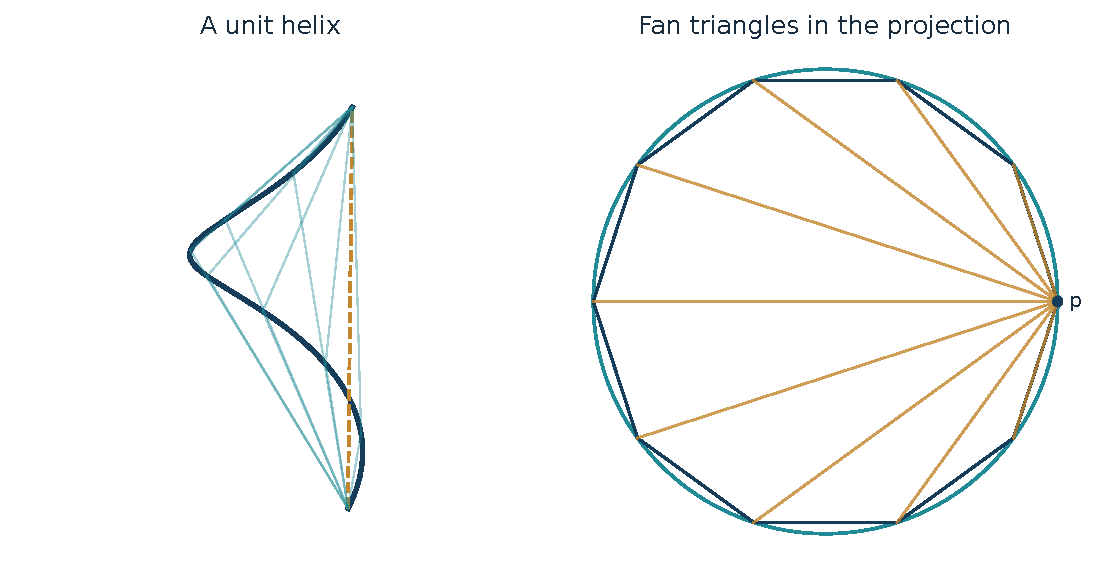
\includegraphics[width=.85\textwidth]{helix.pdf}
\caption{The helix lower bound uses tetrahedra with the two endpoints as a common vertical edge. Their projections are disjoint fan triangles in an inscribed polygon.}
\end{figure}

\clearpage
\bibliographystyle{plainnat}
\bibliography{references}
\end{document}
